% ============================================================
% 1. Introduction
%
% Budget 1.10 pp (1.25 in the structure; the tighter figure is the section's
% share of the running overage). Owns Fig. 1.
%
% SPINE (three-beat reframe, 2026-08-03). The staircase runs on three beats and
% the contribution list is ordered to match them:
%   1. Routing is a feature map on a key producer. Universal: it covers the
%      routed-delta designs too, so no wing split is needed to state it. The
%      family's own self-framings are supporting evidence, not a target.
%   2. The recurrence is a CHOICE, and the literature has routed both. We take
%      linear attention for four positive reasons: it is the class softmax
%      attention itself belongs to (the fold/commutativity material is the
%      IDENTIFICATION of that species, never a boundary drawn against anyone,
%      and it gets ONE sentence with a Sec. 3 pointer); it is efficient in
%      chunked form; it scales to large N; and the delta rule's extra machinery
%      buys nothing when the target, softmax attention, is inside the class,
%      which is what makes the capacity theory the PAYOFF of the choice.
%   3. RoLA is the GENERAL FORM of a routed linear-attention head (the reduction
%      is the constructive theorem behind that phrase), and we build its kernel.
% Registers stay absolute: deflation, no adjudication of the word "attention",
% no universal negatives, no exclusion argument anywhere.
%
% Written last, so every step of the staircase lands on a claim that exists at
% its final strength. Nothing here is stated in result register: Sec. 7's
% measurements are placeholders, so the contributions name derivations
% (the reduction, the capacity theory, the FLOP parity of Eq. 9) and the
% construction, never a measured win.
%
% Fig. 1 is the tradeoff space, not the architecture, and it is schematic:
% the three positions are the structural cost laws of Tab. 1's columns, and
% Sec. 7's Fig. 2 measures the same two axes and places the points.
%
% DUPLICATION SWEEP (claims ledger, D7): fig:space against fig:axis(b) is the
% same pair of axes twice. Both survive (this one earns page 1 as the spine),
% and the caption is cut to the structural laws and the N = L meeting point,
% dropping the two sentences that pre-announced Secs. 6 and 7.
% ============================================================
\section{Introduction}
\label{sec:intro}

Softmax attention retains every token it has read, a key and a value apiece. It scores each query against all of them, so compute per token and stored state both grow with the context \citep{vaswani2017}.

Linear attention bounds both. A feature map that factors the query-key similarity folds the history into a recurrent state of fixed size, so a read is one contraction and nothing accumulates with length \citep{katharopoulos2020}. What it gives up is associative recall. The state is one destination for every write, so the pairs deposited in it lie on top of one another. A query recovers a value only while nothing else has landed where it was stored. Recall explains $82$ percent of the perplexity gap between attention and the gated-convolution models where that gap has been decomposed \citep{arora2023zoology}.

The single destination is the thing to change. That state is one value slot, so provide many and route tokens among them: a token deposits where its content sends it, and a query reads there.

A small instance fixes what that buys. Take a head with three features and a vocabulary of five items, where any one sequence names two of the five and a later query asks for one of the two. If the two live items land in different features, each read returns what was stored. If they land in the same feature, the read returns a blend of the two and nothing downstream can separate them.

What the head has to provision for is therefore the number of items a read must keep apart at once. That is two here, and never the five the vocabulary holds or the length of the sequence that named them. Section~\ref{sec:capacity} turns that count into a graph and the head's size into its chromatic number.

Several architectures of the past year build versions of this, differing in how a token selects slots and how a slot forgets \citep{afzal2026raven, xiao2026ramnet, du2025mom, sse2025, cabannes2026sdm}. Routing is a technique for building keys, a producer of the query and key features that any architecture carrying queries, keys and values needs. A routed design is therefore the recurrence it already ran with a new feature map in front of it.

That reading covers the whole family, and several members place themselves inside linear attention already, each stating it for the one router it builds \citep{sse2025} (Appendix~\ref{apd:ladder}).

What is left to choose is the recurrence, and the literature has routed both linear attention and the delta rule. We take linear attention, for four reasons. It is the class softmax attention itself belongs to: attention's cache appends a key and a value per token and modifies nothing already stored. At $\Nst = L$ it is a member like any other.

What identifies the class is that folding a chunk's transitions into its keys asks them to commute across tokens, so the order they are applied in cannot matter. The delta rule's transitions fail that \citep{schlag2021fwp} (Section~\ref{sec:reduction}). What we are trying to match is softmax attention, which the class contains, so the delta rule's extra machinery buys nothing here.

Working affine is working inside the same species as the architecture to be matched, so parity at matched capacity is a hypothesis. This paper is its test. The capacity theory sizes the state a task demands, the cost arithmetic prices the addressing (Section~\ref{sec:cost}), and Section~\ref{sec:experiments} states the protocol. The rest of the regime arrives with the same affineness. A readout's exactness survives however far a write spread, the backward pass reconstructs no state history, and a per-token bill follows the features a token touches.

\begin{figure}[H]
\centering
\begin{minipage}[b]{0.49\linewidth}
\centering
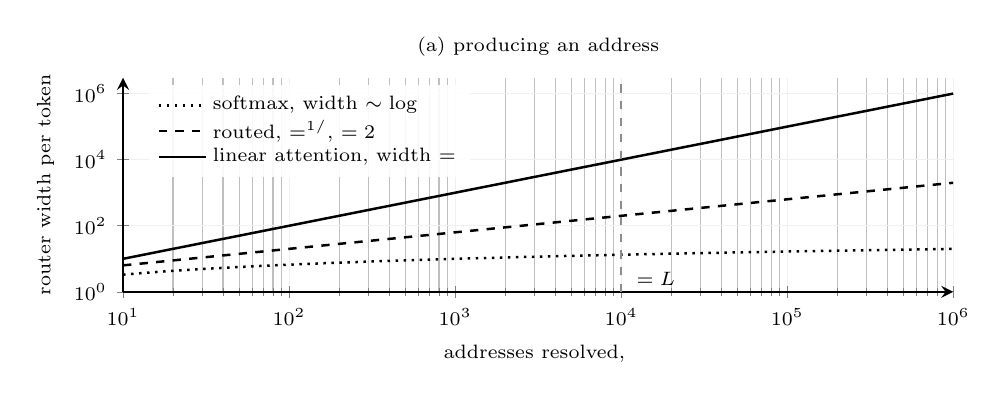
\begin{tikzpicture}
\begin{axis}[
  width=1.0\linewidth, height=4.3cm,
  xmode=log, ymode=log, log basis x=10, log basis y=10,
  domain=10:1e6, samples=60,
  xmin=10, xmax=1e6, ymin=1, ymax=3e6,
  xlabel={addresses resolved, $\Nst$},
  ylabel={router width per token},
  axis lines=left, grid=both, major grid style={gray!12},
  tick label style={font=\scriptsize}, label style={font=\scriptsize},
  legend pos=north west, legend cell align=left,
  legend style={font=\scriptsize, draw=none, fill=white, fill opacity=0.9, text opacity=1, row sep=-2pt},
  title style={font=\scriptsize, yshift=-2pt}, title={(a) producing an address},
  line width=0.9pt,
]
\addplot[black, dotted] {ln(x)/ln(2)};      \addlegendentry{softmax, width $\sim \log \Nst$}
\addplot[black, dashed] {2*sqrt(x)};        \addlegendentry{routed, $\Slv = \Dlv \Nst^{1/\Dlv}$, $\Dlv = 2$}
\addplot[black] {x};                        \addlegendentry{linear attention, width $= \Nst$}
\draw[dashed, black!45] (axis cs:1e4,1) -- (axis cs:1e4,3e6);
\node[font=\scriptsize, anchor=south west, inner sep=1.5pt] at (axis cs:1.15e4,1.1) {$\Nst = L$};
\end{axis}
\end{tikzpicture}
\end{minipage}\hfill
\begin{minipage}[b]{0.49\linewidth}
\centering
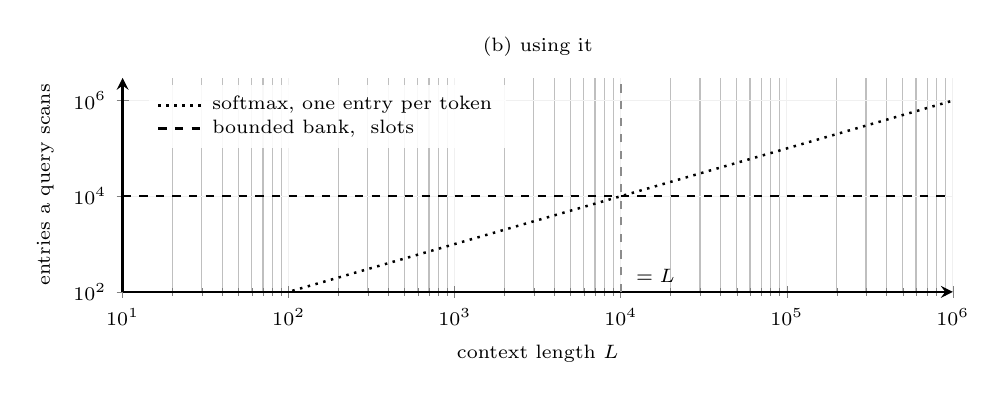
\begin{tikzpicture}
\begin{axis}[
  width=1.0\linewidth, height=4.3cm,
  xmode=log, ymode=log, log basis x=10, log basis y=10,
  domain=10:1e6, samples=60,
  xmin=10, xmax=1e6, ymin=1e2, ymax=3e6,
  xlabel={context length $L$},
  ylabel={entries a query scans},
  axis lines=left, grid=both, major grid style={gray!12},
  tick label style={font=\scriptsize}, label style={font=\scriptsize},
  legend pos=north west, legend cell align=left,
  legend style={font=\scriptsize, draw=none, fill=white, fill opacity=0.9, text opacity=1, row sep=-2pt},
  title style={font=\scriptsize, yshift=-2pt}, title={(b) using it},
  line width=0.9pt,
]
\addplot[black, dotted] {x};                \addlegendentry{softmax, one entry per token}
\addplot[black, dashed] {1e4};              \addlegendentry{bounded bank, $\Nst$ slots}
\draw[dashed, black!45] (axis cs:1e4,1e2) -- (axis cs:1e4,3e6);
\node[font=\scriptsize, anchor=south west, inner sep=1.5pt] at (axis cs:1.15e4,1.2e2) {$\Nst = L$};
\end{axis}
\end{tikzpicture}
\end{minipage}
\caption{\textbf{What an address costs, on both sides.} The abscissa in (a) is the number of slots a design resolves and the ordinate is the router width a token produces to reach them, which is the query--key width for a similarity or a dense feature map and $\Slv = \sum_l \bl$ for a factorized router. Softmax attention's similarity multiplies evidence across dimensions, so $\Theta(\log \Nst)$ features separate $\Nst$ addresses. Linear attention's is a sum over features, so its capacity is the feature dimension itself. A factorized router lies between, at $\Dlv \Nst^{1/\Dlv}$ for fixed depth and logarithmic once depth grows with capacity. Attention is the cheaper producer, and (b) is what it pays for that: its addresses are the tokens themselves, so the entries a query scans grow with the context, where $\Nst$ slots hold whatever the context is. The two meet at $\Nst = L$, where a comparison is capacity-fair (Section~\ref{sec:corner}). The curves are structural laws with constants suppressed.}
\label{fig:space}
\end{figure}

Take a memory whose slots update independently and whose readout is linear, with write and read coefficients that are functions of the input alone. That recurrence is linear attention at feature dimension $\Nst$, its two routing vectors in the roles of key and query features (Section~\ref{sec:reduction}). The statement holds for any router, so it describes the general form of a routed linear-attention head.

RoLA is the head this licenses, and its feature map is factorized. It has $\Dlv$ routing levels, level $l$ offering a choice among $\bl$ branches, with one sparse distribution per level. A leaf is a complete address, one branch chosen at every level, and it names one slot.

Capacity is then the product of the widths where the router's output is their sum, $\prod_l \bl$ slots from $\sum_l \bl$ numbers, which is the mixed-radix arithmetic the design runs on.

The contributions follow that order.
\begin{enumerate}\setlength{\itemsep}{1pt}\setlength{\parskip}{0pt}
\item The reduction, and the recent routed family located in it, including the update rules that fall outside it (Section~\ref{sec:reduction}).
\item The capacity theory that sizes $\Nst$ against what a retrieval contract demands, with the rule that a comparison matches addressing entropy, the log of the number of addresses a design resolves, in place of parameter count (Section~\ref{sec:capacity}). Addressing entropy is, in short, how many distinct places a design can tell apart, counted in bits.
\item The hierarchical entmax feature map, in the three wirings of its read and write supports. Its decay runs on a clock of received write mass, learned per level and held off the gradient, which is what removes the state history from the backward pass (Section~\ref{sec:rola}).
\item The kernel that bills the slots a token touches and not the slots it owns, with the cost model that plans it. It runs at $\Nst = 65{,}536$ and meets attention's arithmetic at $\Nst = L$ (Section~\ref{sec:cost}).
\end{enumerate}

The released layer takes the levels, their widths, each level's activation and side assignment, and the clock as configuration (Appendix~\ref{apd:ladder}).

Language modelling at any scale is the sequel's subject.
